\documentclass[lang=cn,11pt,a4paper,cite=authornum]{paper}

\title{计算机网络实验二:网络层数据分组的捕获和解析\ 实验报告}
\author{毛子恒 \\ 2019211397}
\institute{北京邮电大学\ 计算机学院}

\date{\zhtoday}

% 本文档命令
\usepackage{array}
\newcommand{\ccr}[1]{\makecell{{\color{#1}\rule{1cm}{1cm}}}}
\nocite{*}

\begin{document}

\maketitle

\section{实验内容和实验环境描述}

\subsection{实验内容}

本次实验内容:

\begin{enumerate}
    \item 捕获在连接Internet过程中产生的网络层分组:DHCP分组,ARP分组,IP数据分组,ICMP分组。
    \item 分析各种分组的格式,说明各种分组在建立网络连接过程中的作用。
    \item 分析IP数据分组分片的结构。
\end{enumerate}

通过本次实验了解计算机上网的工作过程,学习各种网络层分组的格式及其作用,理解长度大于1500字节IP数据组分片传输的结构。

\subsection{实验环境}

\begin{itemize}
    \item Windows 10 version 1909
    \item Wireshark Version 3.4.4
    \item Visual Studio Code 1.56.2
\end{itemize}

\section{实验步骤和网络层分组结构分析}

\subsection{准备工作}

启动计算机,连接网络确保能够上网。断开连接,禁用网卡。

\subsection{捕获和分析DHCP和ARP分组}

\subsubsection{捕获DHCP分组}

开启监控,连接网络。在Wireshark过滤器中输入\mintinline{shell}{dhcp},过滤出四个DHCP分组如\figref{fig:dhcps}。

\begin{figure}[htbp]

    \centering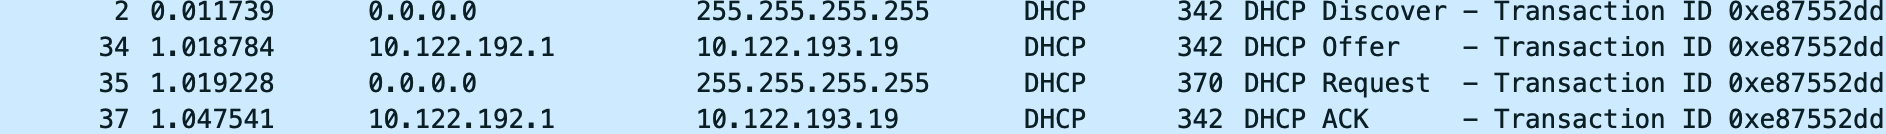
\includegraphics[width=\textwidth]{./Images/DHCPS.png}

    \caption{捕获到的四个DHCP分组\label{fig:dhcps}}

\end{figure}

四个DHCP分组的内容如\figref{fig:dhcp}。

\begin{figure}[htbp]

    \centering
    
    \subfigure[DHCP Discover]{
        \begin{minipage}[t]{0.45\linewidth}
            \centering
            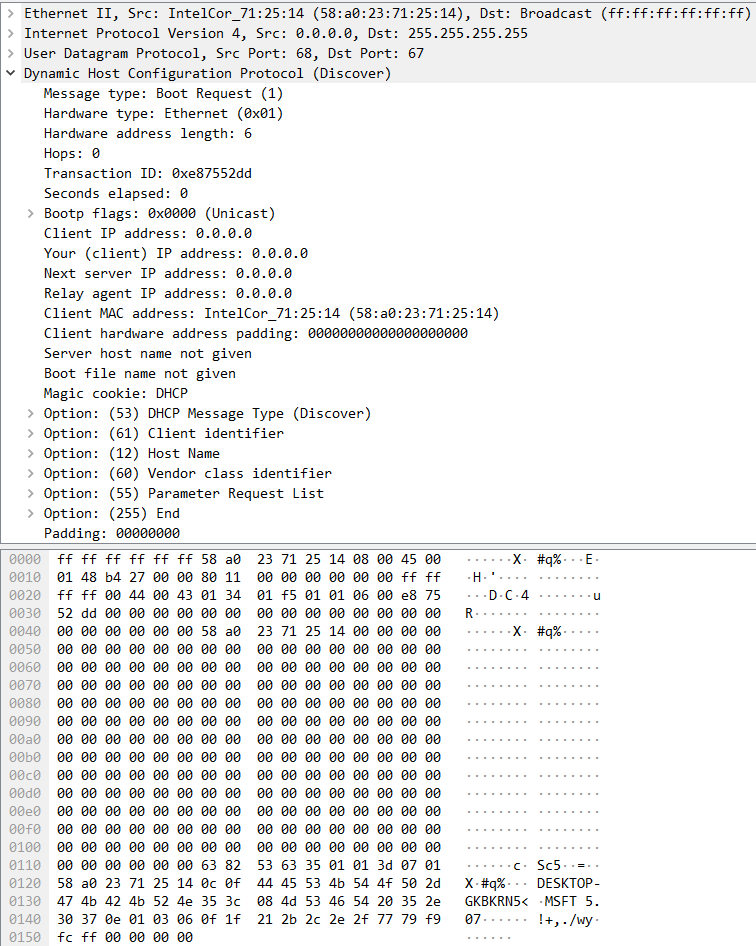
\includegraphics[width=\linewidth]{./Images/DHCP1.png}
        \end{minipage}
    }
    \subfigure[DHCP Offer]{
        \begin{minipage}[t]{0.45\linewidth}
            \centering
            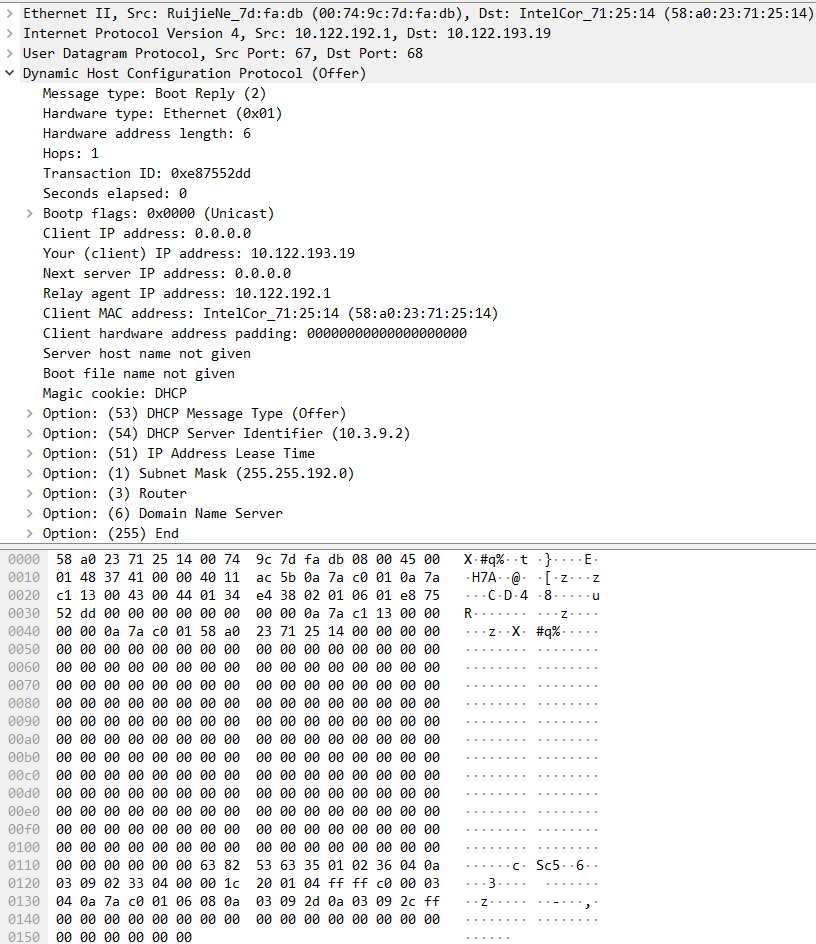
\includegraphics[width=\linewidth]{./Images/DHCP2.png}
        \end{minipage}
    }
    
    \subfigure[DHCP Request]{
        \begin{minipage}[t]{0.45\linewidth}
            \centering
            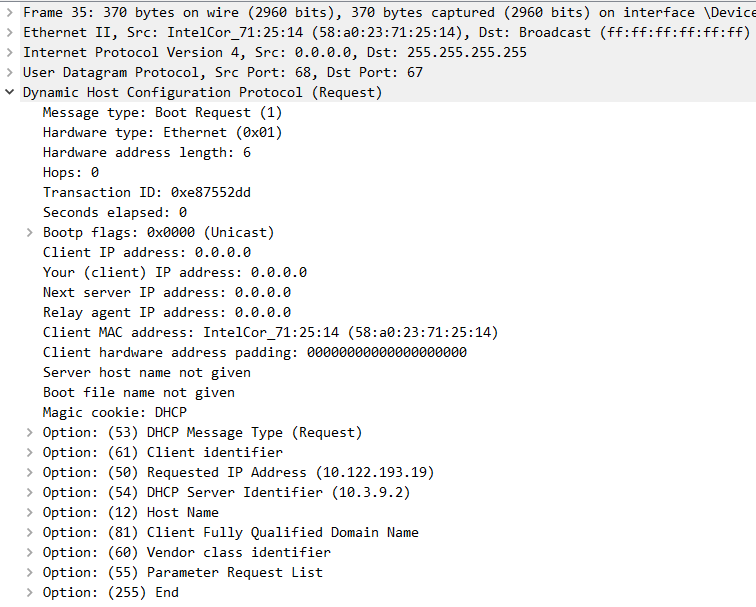
\includegraphics[width=\textwidth]{./Images/DHCP3-1.png}
            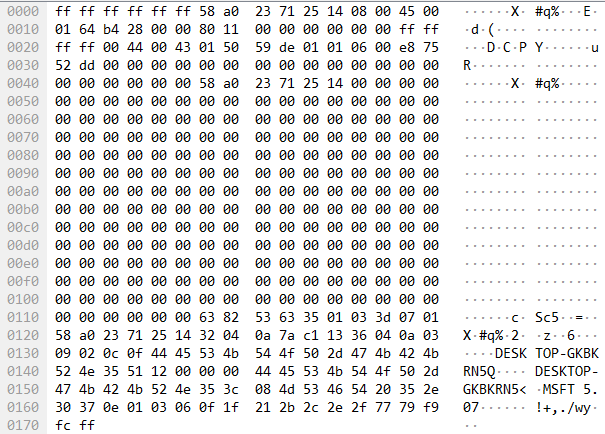
\includegraphics[width=\textwidth]{./Images/DHCP3-2.png}
        \end{minipage}
    }
    \subfigure[DHCP ACK]{
        \begin{minipage}[t]{0.45\linewidth}
            \centering
            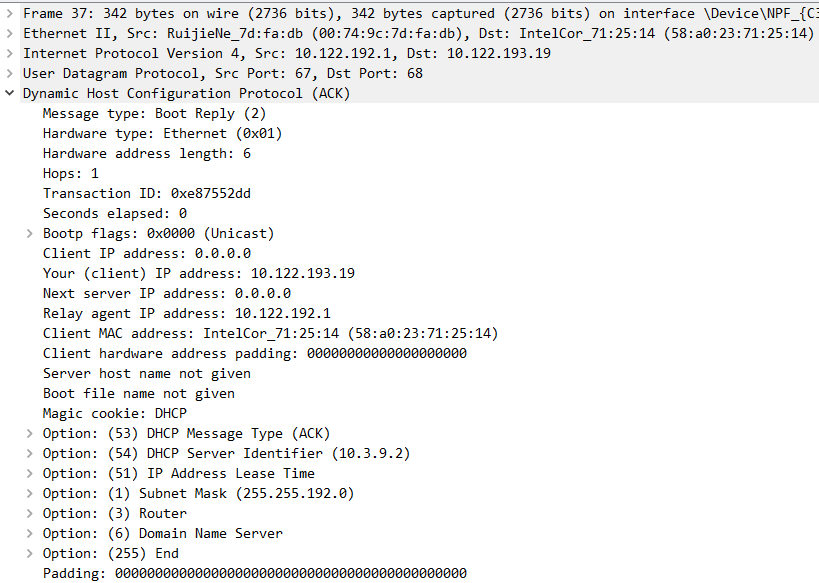
\includegraphics[width=\textwidth]{./Images/DHCP4-1.png}
            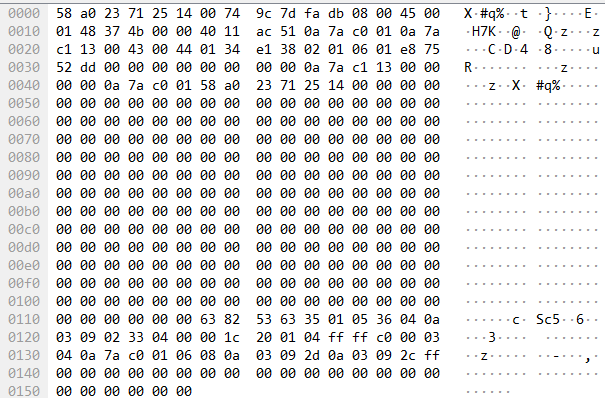
\includegraphics[width=\textwidth]{./Images/DHCP4-2.png}
        \end{minipage}
    }
    \caption{四个DHCP分组的内容\label{fig:dhcp}}

\end{figure}

\subsubsection{分析DHCP分组}

序号为2的DHCP分组内容的分析如\tabref{tab:dhcp1res}。

\begin{table}[!htbp]
    \centering
    \caption{DHCP Discover分组内容分析\label{tab:dhcp1res}}
    \begin{tabular}{|c|c|l|}
        \hline
        字段 (字节数) & 内容(16进制) & 解释 \\
        \hline
        OP (1) & 01 & 消息类型:引导请求 \\
        \hline
        HTYPE (1) & 01 & 硬件地址类型:以太网 \\
        \hline
        HLEN (1) & 06 & 硬件地址长度:6 \\
        \hline
        HOPS (1) & 00 & 经过的DHCP中继的数目:0 \\
        \hline
        XID (4) & e8 75 52 dd & 处理ID,标记一次IP地址请求过程:0xe87552dd \\
        \hline
        SECS (2) & 00 00 & 从获取到IP地址或者续约过程开始到现在所消耗的时间:0秒 \\
        \hline
        FLAGS (2) & 00 00 & 标记:第一位为0,表示单播 \\
        \hline
        CIADDR (4) & 00 00 00 00 & \makecell[l]{客户端IP地址:0.0.0.0 \\ 还未分配IP地址} \\
        \hline
        YIADDR (4) & 00 00 00 00 & \makecell[l]{你的(客户端)IP地址(服务器分配的地址):0.0.0.0 \\ 仅在Offer和ACK分组中有效} \\
        \hline
        SIADDR (4) & 00 00 00 00 & \makecell[l]{在bootstrap过程中下一台服务器的地址:0.0.0.0 \\ DHCP服务器未知} \\
        \hline
        GIADDR (4) & 00 00 00 00 & \makecell[l]{客户端发出请求分组后经过的第一个中继的地址:0.0.0.0 \\ 没有经过中继} \\
        \hline
        CHADDR (16) & 58 a0 23 71 25 14 & \makecell[l]{客户端的MAC地址:58:a0:23:71:25:14 \\ 后接10个字节的填充} \\
        \hline
        SNAME (64) & 全部为00 & 为客户端分配IP地址的服务器域名:未给出 \\
        \hline
        FILE (128) & 全部为00 & 为启动客户端指定的配置文件路径:未给出 \\
        \hline
        \makecell[c]{magic \\ cookie(4)} & 63 82 53 63 & 可选字段的格式:DHCP \\
        \hline
        OPTION (3) & 35 01 01 & DHCP消息类型:Discover \\
        \hline
        OPTION (9) & \makecell[c]{3d 07 01 \\ 58 a0 23 71 25 14} & 客户端标识符:以太网,MAC地址58:a0:23:71:25:14 \\
        \hline
        OPTION (17) & 0c 0f 后略 & 主机名,长度为15 \\
        \hline
        OPTION (8) & 3c 08 后略 & 供应商标识符,长度为8 \\
        \hline
        OPTION (16) & 37 0e 后略 & 参数需求列表,长度为14 \\
        \hline
        OPTION (1) & ff & 选项字段结束 \\
        \hline
    \end{tabular}
\end{table}

序号为34、35、37的DHCP分组内容的分析如\tabref{tab:dhcp2res}、\tabref{tab:dhcp3res}和\tabref{tab:dhcp4res},表中仅展示与第一个分组不同的部分。

\begin{table}[!htbp]
    \centering
    \caption{DHCP Offer分组内容分析\label{tab:dhcp2res}}
    \begin{tabular}{|c|c|l|}
        \hline
        字段 (字节数) & 内容(16进制) & 解释 \\
        \hline
        OP (1) & 02 & 消息类型:引导回复 \\
        \hline
        HOPS (1) & 01 & 经过的DHCP中继的数目:1 \\
        \hline
        YIADDR (4) & 0a 7a c1 13 & 你的(客户端)IP地址(服务器分配的地址):10.122.193.19 \\
        \hline
        GIADDR (4) & 0a 7a c0 01 & 客户端发出请求分组后经过的第一个中继的地址:10.122.192.1 \\
        \hline
        OPTION (3) & 35 01 02 & DHCP消息类型:Offer \\
        \hline
        OPTION (6) & 36 04 0a 03 09 02 & DHCP服务器标识符:10.3.9.2 \\
        \hline
        OPTION (6) & 33 04 00 00 1c 20 & IP地址释放时间:7200秒 \\
        \hline
        OPTION (6) & 01 04 ff ff c0 00 & 子网掩码:255.255.192.0 \\
        \hline
        OPTION (6) & 03 04 0a 7a c0 01 & 路由器:10.122.192.1 \\
        \hline
        OPTION (10) & \makecell[c]{06 08 0a 03 09 2d \\ 0a 03 09 2c} & 域名服务器:10.3.9.45、10.3.9.44 \\
        \hline
        OPTION (1) & ff & 选项字段结束 \\
        \hline
    \end{tabular}
\end{table}

\begin{table}[!htbp]
    \centering
    \caption{DHCP Request分组内容分析\label{tab:dhcp3res}}
    \begin{tabular}{|c|c|l|}
        \hline
        字段 (字节数) & 内容(16进制) & 解释 \\
        \hline
        OPTION (3) & 35 01 03 & DHCP消息类型:Request \\
        \hline
        OPTION (9) & \makecell[c]{3d 07 01 \\ 58 a0 23 71 25 14} & 客户端标识符:以太网,MAC地址58:a0:23:71:25:14 \\
        \hline
        OPTION (6) & 32 04 0a 7a c1 13 & 请求的IP地址:10.122.193.19 \\
        \hline
        OPTION (6) & 36 04 0a 03 09 02 & DHCP服务器标识符:10.3.9.2 \\
        \hline
        \multicolumn{3}{|c|}{省略一部分选项字段} \\ 
        \hline
        OPTION (1) & ff & 选项字段结束 \\
        \hline
    \end{tabular}
\end{table}

\begin{table}[!htbp]
    \centering
    \caption{DHCP ACK分组内容分析\label{tab:dhcp4res}}
    \begin{tabular}{|c|c|l|}
        \hline
        字段 (字节数) & 内容(16进制) & 解释 \\
        \hline
        OP (1) & 02 & 消息类型:引导回复 \\
        \hline
        HOPS (1) & 00 & 经过的DHCP中继的数目:1 \\
        \hline
        YIADDR (4) & 0a 7a c1 13 & 你的(客户端)IP地址(服务器分配的地址):10.122.193.19 \\
        \hline
        GIADDR (4) & 0a 7a c0 01 & 客户端发出请求分组后经过的第一个中继的地址:10.122.192.1 \\
        \hline
        OPTION (3) & 35 01 05 & DHCP消息类型:ACK \\
        \hline
        \multicolumn{3}{|c|}{省略一部分选项字段} \\ 
        \hline
        OPTION (1) & ff & 选项字段结束 \\
        \hline
    \end{tabular}
\end{table}

\subsubsection{分析DHCP的工作流程}

DHCP协议用于对连接到网络的设备自动分配IP地址和其他通信变量。

\begin{enumerate}
    \item 客户端连入局域网后,向局域网内发送广播,发送一个DHCP Discover分组,分组内容中有本机的MAC地址,并在OPTION字段中附带一个请求参数的列表。
    \item 服务器为客户端分配IP,并向之前的MAC地址发送DHCP Offer分组,分组内容中有分配的IP地址,分组的OPTION字段中附带服务器标识符、IP租期、子网掩码等信息。
    \item 客户端再次发送广播,发送一个DHCP Request分组,在OPTIONS字段中指明请求的IP地址和服务器标识符。
    \item 服务器向客户端发送DHCP ACK分组确认。
\end{enumerate}

\subsubsection{捕获ARP分组}

在Wireshark过滤器中输入\mintinline{shell}{arp},过滤出数个ARP分组。分组的内容如\figref{fig:arp}。

\begin{figure}[htbp]

    \centering
    
    \subfigure[序号36的ARP分组]{
        \begin{minipage}[t]{0.45\linewidth}
            \centering
            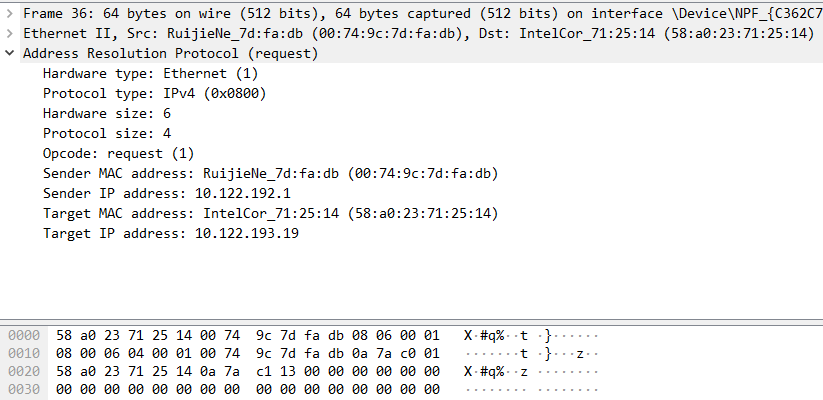
\includegraphics[width=\linewidth]{./Images/ARP1.png}
        \end{minipage}
    }
    \subfigure[序号59的ARP分组]{
        \begin{minipage}[t]{0.45\linewidth}
            \centering
            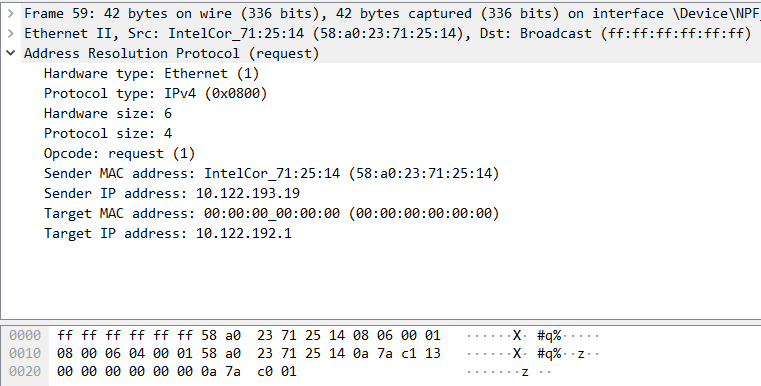
\includegraphics[width=\linewidth]{./Images/ARP2.png}
        \end{minipage}
    }
    
    \subfigure[序号64的ARP分组]{
        \begin{minipage}[t]{0.45\linewidth}
            \centering
            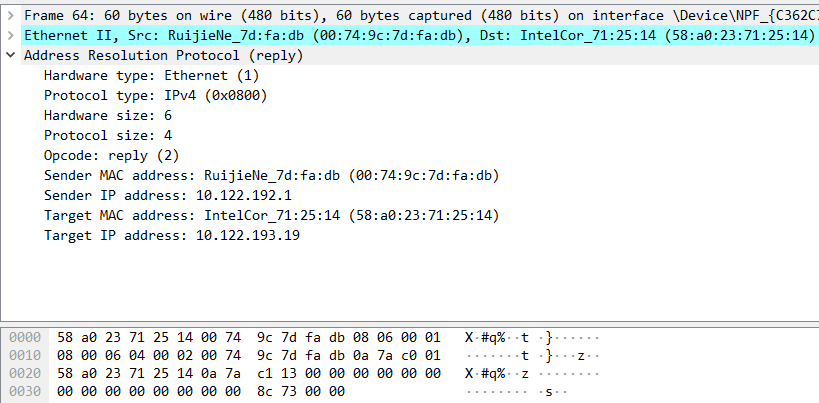
\includegraphics[width=\textwidth]{./Images/ARP3.png}
        \end{minipage}
    }
    \subfigure[序号71的ARP分组]{
        \begin{minipage}[t]{0.45\linewidth}
            \centering
            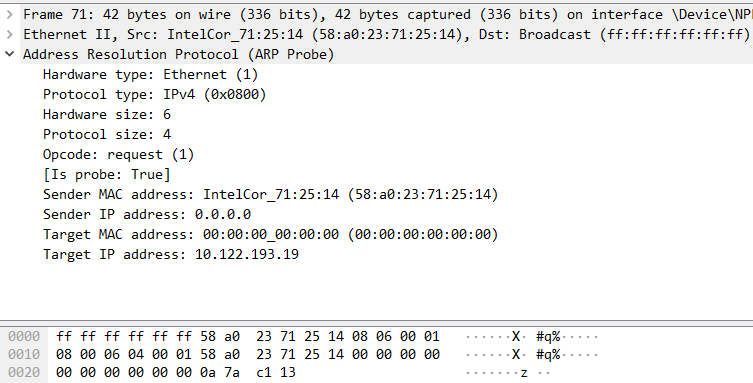
\includegraphics[width=\textwidth]{./Images/ARP4.png}
        \end{minipage}
    }

    \subfigure[序号255的ARP分组]{
        \begin{minipage}[t]{0.45\linewidth}
            \centering
            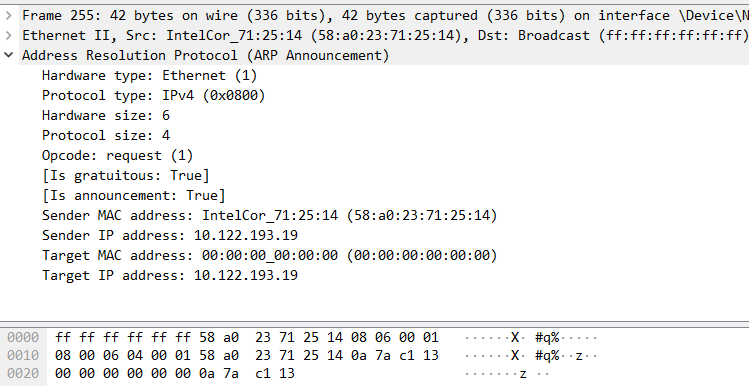
\includegraphics[width=\textwidth]{./Images/ARP5.png}
        \end{minipage}
    }
    \subfigure[序号315的ARP分组]{
        \begin{minipage}[t]{0.45\linewidth}
            \centering
            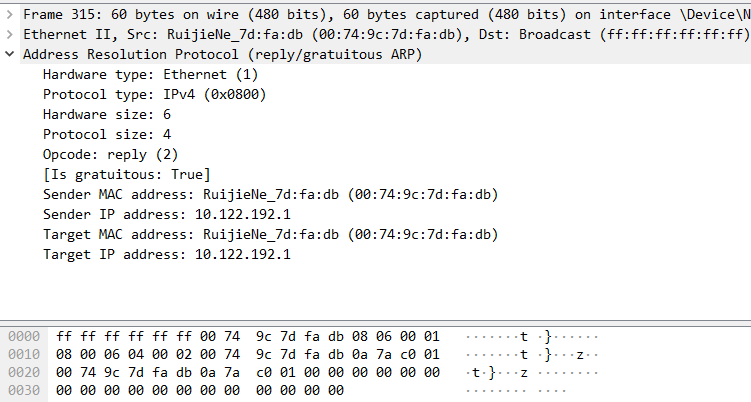
\includegraphics[width=\textwidth]{./Images/ARP6.png}
        \end{minipage}
    }
    \caption{ARP分组的内容\label{fig:arp}}

\end{figure}

\subsubsection{分析ARP分组}

序号为36的ARP分组内容的分析如\tabref{tab:arpres}。

\begin{table}[!htbp]
    \centering
    \caption{序号为36的ARP分组内容分析\label{tab:arpres}}
    \begin{tabular}{|c|c|l|}
        \hline
        字段 (字节数) & 内容(16进制) & 解释 \\
        \hline
        HTYPE (2) & 00 01 & 硬件类型:以太网 \\
        \hline
        PTYPE (2) & 08 00 & 协议类型:IPv4 \\
        \hline
        HLEN (1) & 06 & 硬件地址长度:6 \\
        \hline
        PLEN (1) & 04 & 协议地址长度:4 \\
        \hline
        OPER (2) & 00 01 & ARP消息类型:request \\
        \hline
        SHA (6) & 00 74 9c 7d fa db & 发送方MAC地址:00:74:9c:7d:fa:db \\
        \hline
        SPA (4) & 0a 7a c0 01 & 发送方IP地址:10.122.192.1 \\
        \hline
        THA (6) & 58 a0 23 71 25 14 & 接收方MAC地址:58:a0:23:71:25:14 \\
        \hline
        TPA (6) & 0a 7a c1 13 & 接收方IP地址:10.122.193.19 \\
        \hline
    \end{tabular}
\end{table}

\subsubsection{分析ARP的工作流程}

ARP协议用于将网络层地址(比如IPv4),映射到链路层地址(比如MAC)。

\begin{enumerate}
    \item 序号为36的ARP分组发送在DHCP Request和DHCP ACK之间,此时路由器请求10.122.193.19的MAC地址,但是此时IP地址还没有分配,所以本机没有回复。
    \item 序号为59的ARP分组发送在IP地址分配完成之后,本机向局域网发送广播,请求10.122.192.1,即路由器的MAC地址。
    \item 序号为64的ARP分组是对第二个ARP的回复,其中OPER字段设为2,表示一个回复分组,分组内容中发送方的部分为路由器的IP和MAC地址。
    \item 序号为71的ARP分组是一个ARP探针(ARP Probe)分组,意图是探测IP地址在局域网中是否已经被使用,其发送方MAC地址被设为本机,发送方IP地址和接收方MAC地址被设为空,接收方IP地址设为想要探测的IP地址,即本机的IP地址。
    \item 序号为255的ARP分组是一个ARP声明(ARP Announcement)分组,意图是在局域网中“声明”这个IP地址,除了发送方IP地址被设为本机IP之外,其他内容和ARP Probe分组相同,其他主机可以用发送方IP和MAC地址在ARP缓存中建立映射。
    \item 序号为315的ARP分组是一个免费ARP(Gratuitous ARP)分组,分组中OPER字段设为2(但是并不意味着对某个请求的回复),发送方MAC与接收方MAC相同、发送方IP与接收方IP相同。路由器向局域网广播这个分组,用于让主机更新ARP缓存中的映射。
\end{enumerate}

\subsection{捕获和分析IP分组}

\subsubsection{捕获IP分组}

任意捕获一个IP分组,如\figref{fig:ip0}。

\begin{figure}[htbp]
    \centering
    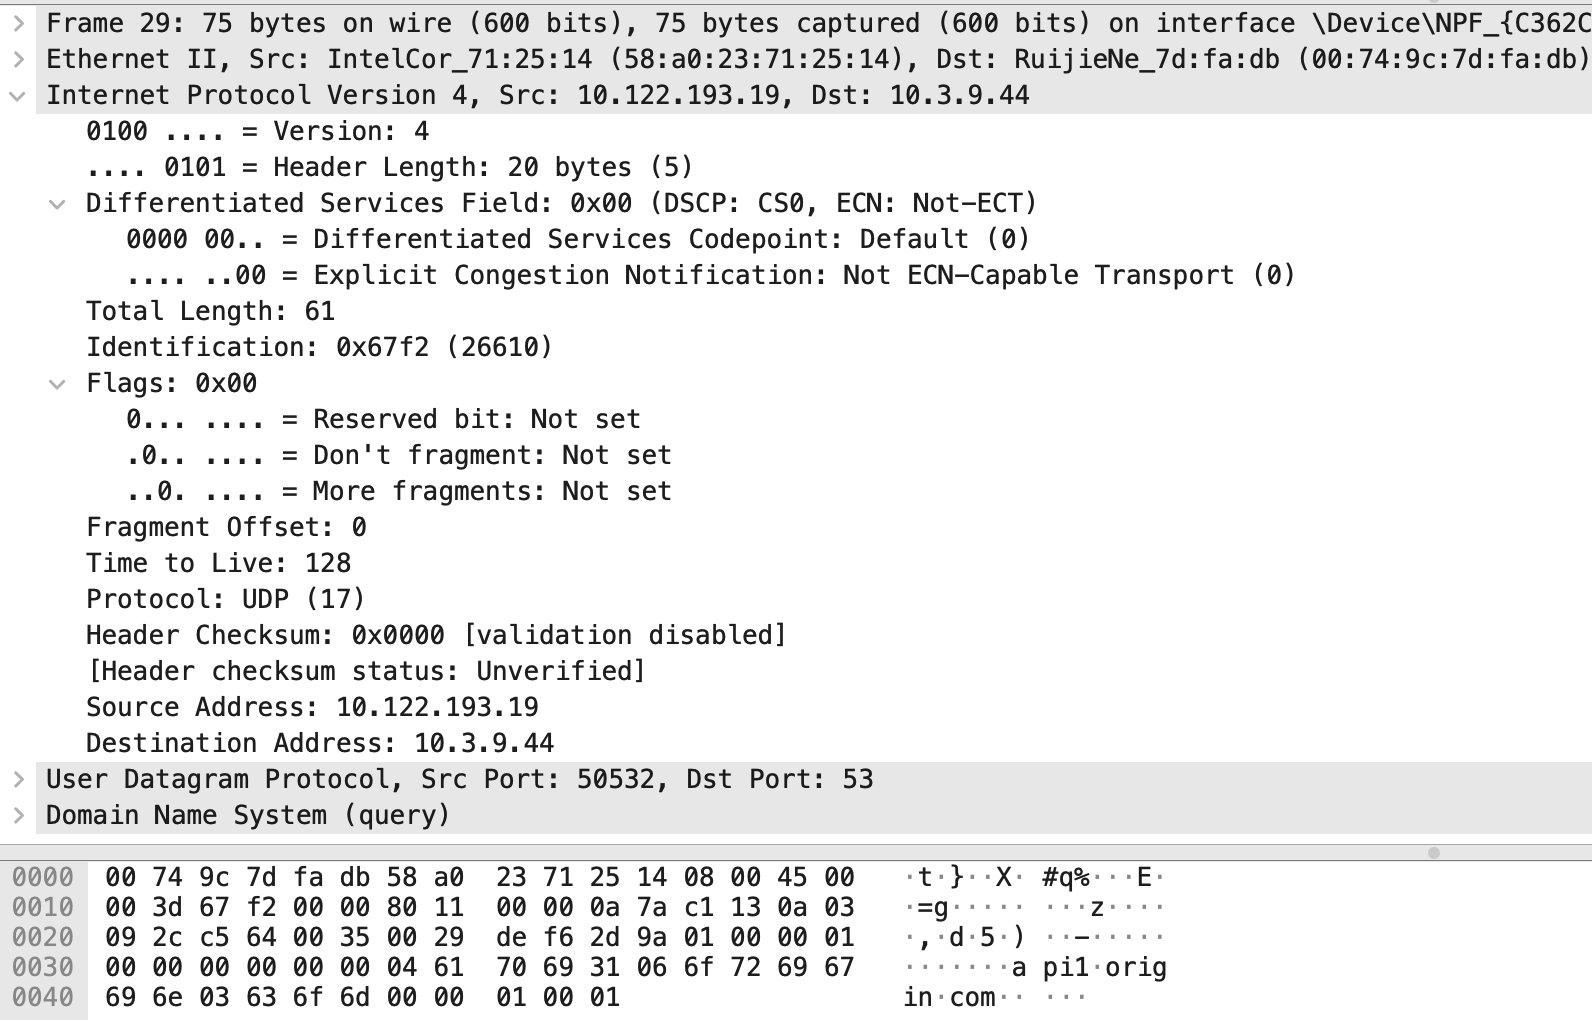
\includegraphics[width=0.7\linewidth]{./Images/IP0.png}
    \caption{序号为29的IP分组\label{fig:ip0}}
\end{figure}

\subsubsection{分析IP分组}

IP分组的分析如\tabref{tab:ip0res}。

\begin{table}[!htbp]
    \centering
    \caption{序号为29的IP分组头分析\label{tab:ip0res}}
    \begin{tabular}{|c|c|l|}
        \hline
        字段 (位数) & 内容(默认16进制) & 解释 \\
        \hline
        Version (4) & 0100B & 版本:4 \\
        \hline
        IHL (4) & 0101B & 头部长度:20字节 \\
        \hline
        DSCP (6) & 000000B & 区分服务信息:默认 \\
        \hline
        ECN (2) & 00B & 显式拥塞通知:否 \\
        \hline
        Total Length (16) & 00 3d & 分组总长度:61字节 \\
        \hline
        Identification (16) & 67 f2 & 分组标识:0x67f2 \\
        \hline
        Flags (3) & 000B & \makecell[l]{Don't Fragment(不要分段)标志位:0 \\ More Fragments(更多的段)标志位:0} \\
        \hline
        Fragment Offset (13) & 0000000000000B & 分段偏移量:0 \\
        \hline
        TTL (8) & 80 & 生存期:128跳 \\
        \hline
        Protocol (8) & 11 & 协议:UDP \\
        \hline
        Header CheckSum (32) & 00 00 00 00 & 头校验和:不验证 \\
        \hline
        Source IP Address (32) & 0a 7a c1 13 & 源地址:10.122.193.19 \\
        \hline
        Destimation IP Address (32) & 0a 03 09 2c & 目标地址:10.3.9.44 \\
        \hline
    \end{tabular}
\end{table}

数据部分是UDP分组和DNS查询分组,略。

\subsubsection{捕获长IP分组}

获取连接到BUPT-mobile的手机的IP地址为10.21.245.157。

在cmd中输入指令\mintinline{shell}{ping 10.21.245.157 -n 1 -l 8000},向手机发送一个长度为8000的IP数据包。

运行结果如\figref{fig:ping}。

\begin{figure}[htbp]
    \centering
    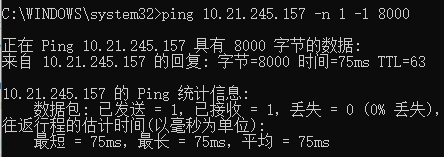
\includegraphics[width=0.5\linewidth]{./Images/ping.png}
    \caption{\mintinline{shell}{ping}指令运行结果\label{fig:ping}}
\end{figure}

在Wireshark过滤器中输入\mintinline{shell}{ip.src eq 10.122.193.19 or ip.dst eq 10.122.193.19},过滤出12个分组如\figref{fig:ips}。

\begin{figure}[htbp]
    \centering
    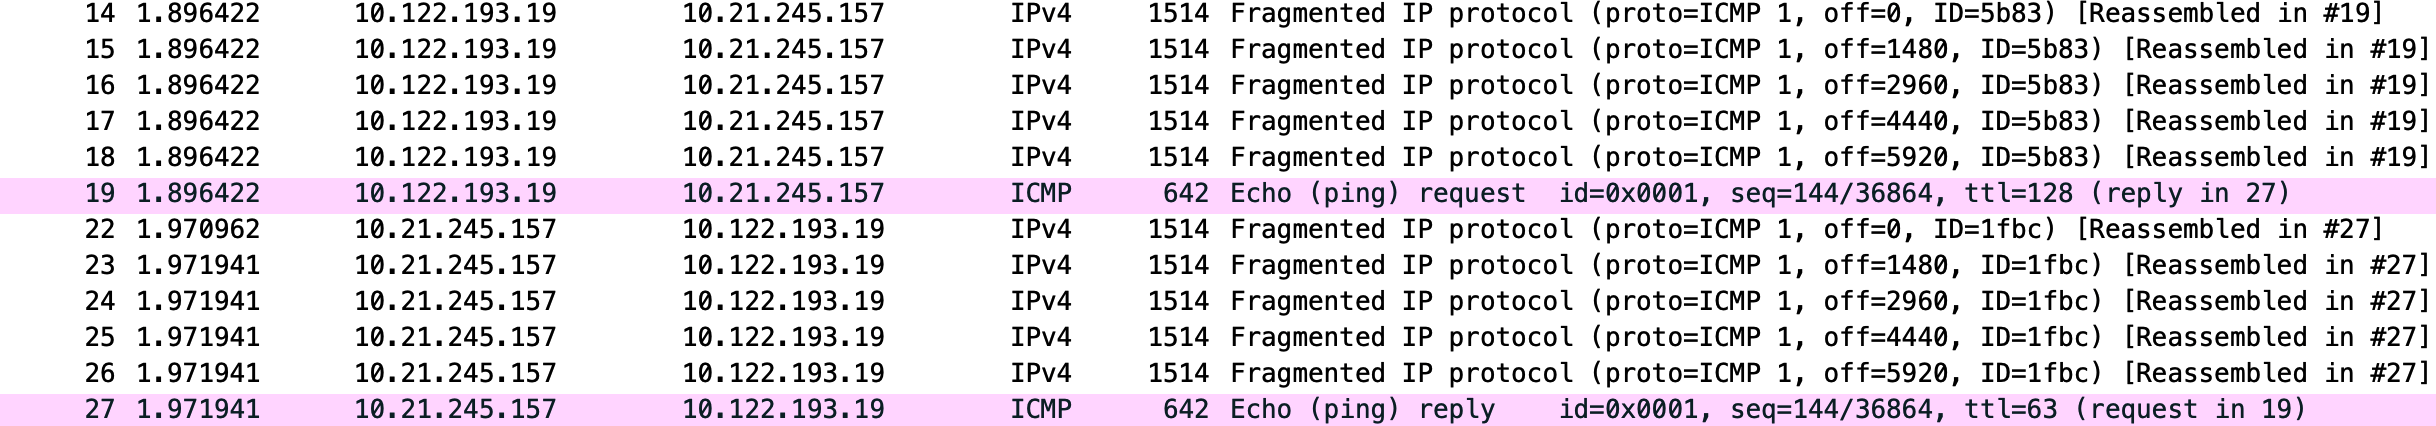
\includegraphics[width=\linewidth]{./Images/IP.png}
    \caption{捕获到的12个IP分组\label{fig:ips}}
\end{figure}

限于篇幅原因,仅展示序号为14的IP分组的内容,如\figref{fig:ip1}。

\begin{figure}[htbp]
    \centering
    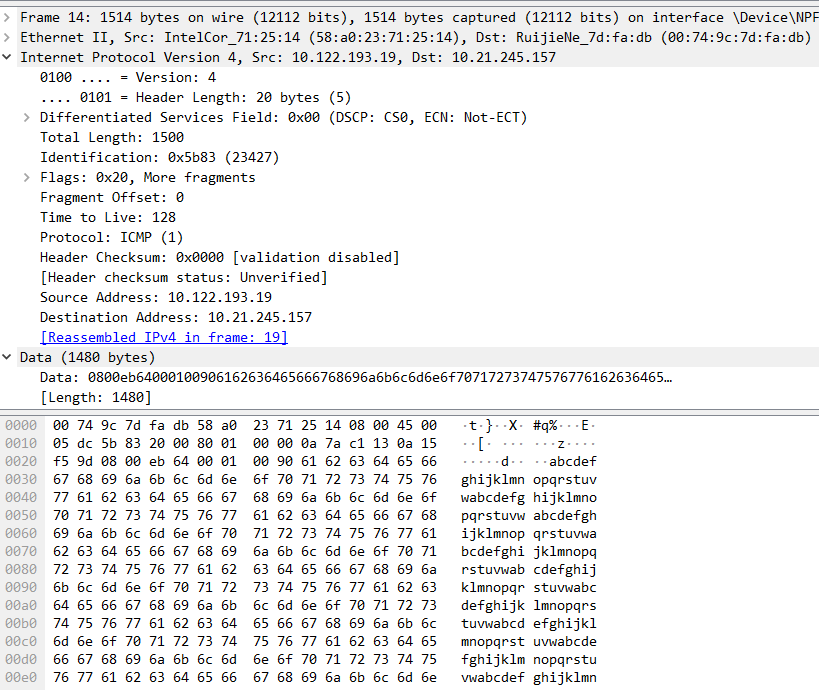
\includegraphics[width=0.7\linewidth]{./Images/IP1.png}
    \caption{序号为14的IP分组的内容\label{fig:ip1}}
\end{figure}

\subsubsection{分析长IP分组}

序号为14的IP分组的分组头部分的分析如\tabref{tab:ip1res}。

\begin{table}[!htbp]
    \centering
    \caption{序号为14的IP分组头分析\label{tab:ip1res}}
    \begin{tabular}{|c|c|l|}
        \hline
        字段 (位数) & 内容(默认16进制) & 解释 \\
        \hline
        Version (4) & 0100B & 版本:4 \\
        \hline
        IHL (4) & 0101B & 头部长度:20字节 \\
        \hline
        DSCP (6) & 000000B & 区分服务信息:默认 \\
        \hline
        ECN (2) & 00B & 显式拥塞通知:否 \\
        \hline
        Total Length (16) & 05 dc & 分组总长度:1500字节 \\
        \hline
        Identification (16) & 5b 83 & 分组标识:0x5b83 \\
        \hline
        Flags (3) & 001B & \makecell[l]{Don't Fragment(不要分段)标志位:0 \\ More Fragments(更多的段)标志位:1} \\
        \hline
        Fragment Offset (13) & 0000000000000B & 分段偏移量:0 \\
        \hline
        TTL (8) & 80 & 生存期:128跳 \\
        \hline
        Protocol (8) & 01 & 协议:ICMP \\
        \hline
        Header CheckSum (32) & 00 00 00 00 & 头校验和:不验证 \\
        \hline
        Source IP Address (32) & 0a 7a c1 13 & 源地址:10.122.193.19 \\
        \hline
        Destimation IP Address (32) & 0a 15 f5 9d & 目标地址:10.21.245.157 \\
        \hline
    \end{tabular}
\end{table}

前六个分组的分组头的大部分内容都一致,它们的MF标志位以及分段偏移量的对比如\tabref{tab:ipcomp}。

\begin{table}[!htbp]
    \centering
    \caption{IP分组头对比\label{tab:ipcomp}}
    \begin{tabular}{|c|c|c|}
        \hline
        分组序号 & MF标志位 & 分段偏移量 \\
        \hline
        14 & 1 & 0 \\
        \hline
        15 & 1 & $185\times8=1480$ \\
        \hline
        16 & 1 & $370\times8=2960$ \\
        \hline
        17 & 1 & $555\times8=4440$ \\
        \hline
        18 & 1 & $740\times8=5920$ \\
        \hline
        19 & 0 & $925\times8=7400$ \\
        \hline
    \end{tabular}
\end{table}

由于以太网数据链路层的MTU为1500字节,除去头之后剩余1480字节,正好是8的倍数,因此长度为8000字节的数据被拆分成6个分段,前五个的长度为1480字节,最后一个的长度为600字节,分段偏移量表示该分段在原数据段中的位置,通过MF标志位为0确定数据的结束。

\subsection{捕获和分析ICMP分组}

\subsubsection{分析ping命令产生的ICMP分组}

\mintinline{shell}{ping}命令产生的ICMP分组的内容如\figref{fig:icmp}。

\begin{figure}[htbp]

    \centering
    
    \subfigure[序号为19的ICMP分组]{
        \begin{minipage}[t]{0.45\linewidth}
            \centering
            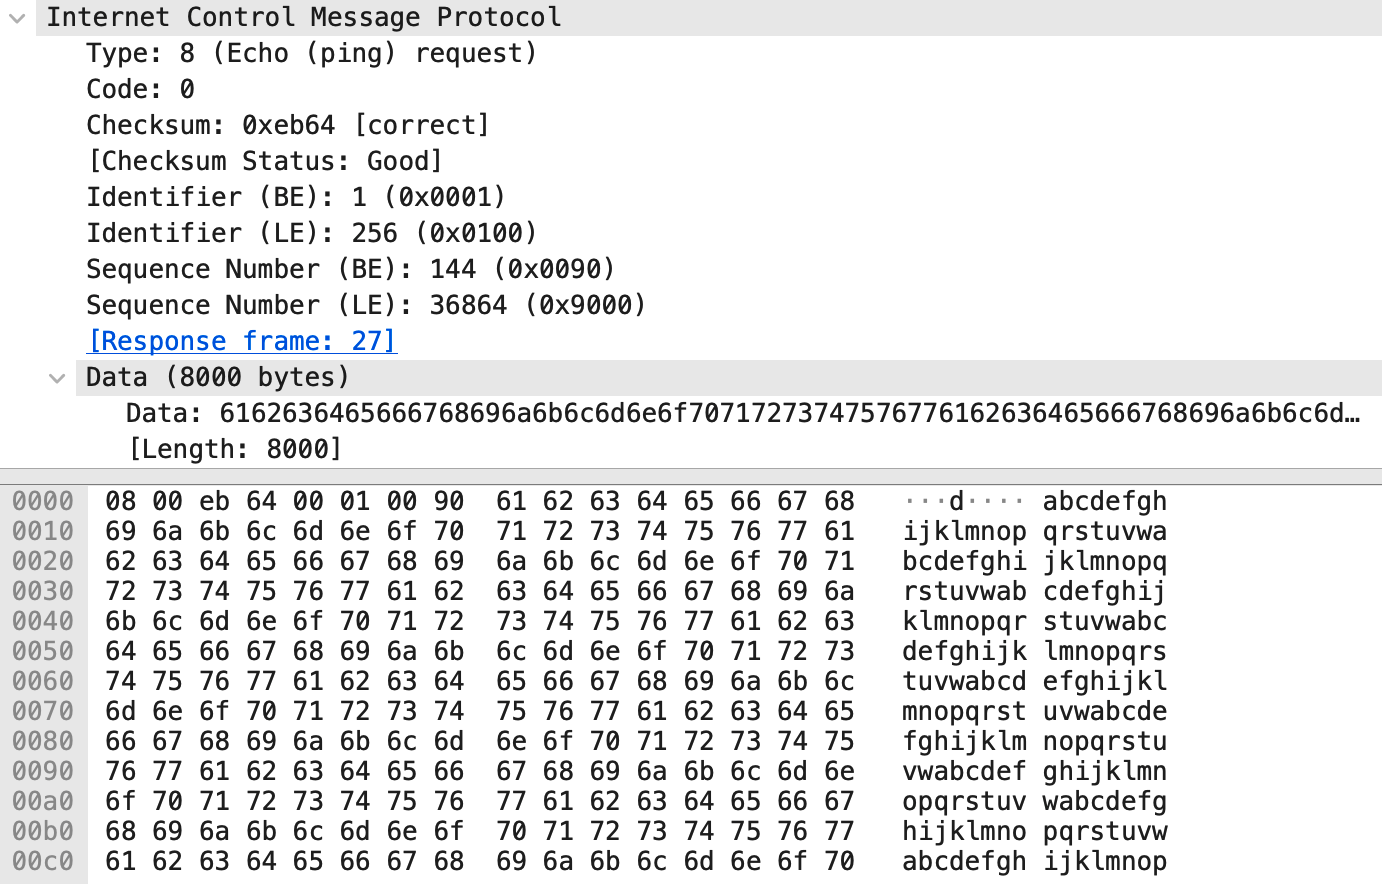
\includegraphics[width=\linewidth]{./Images/ICMP1.png}
        \end{minipage}
    }
    \subfigure[序号为27的ICMP分组]{
        \begin{minipage}[t]{0.45\linewidth}
            \centering
            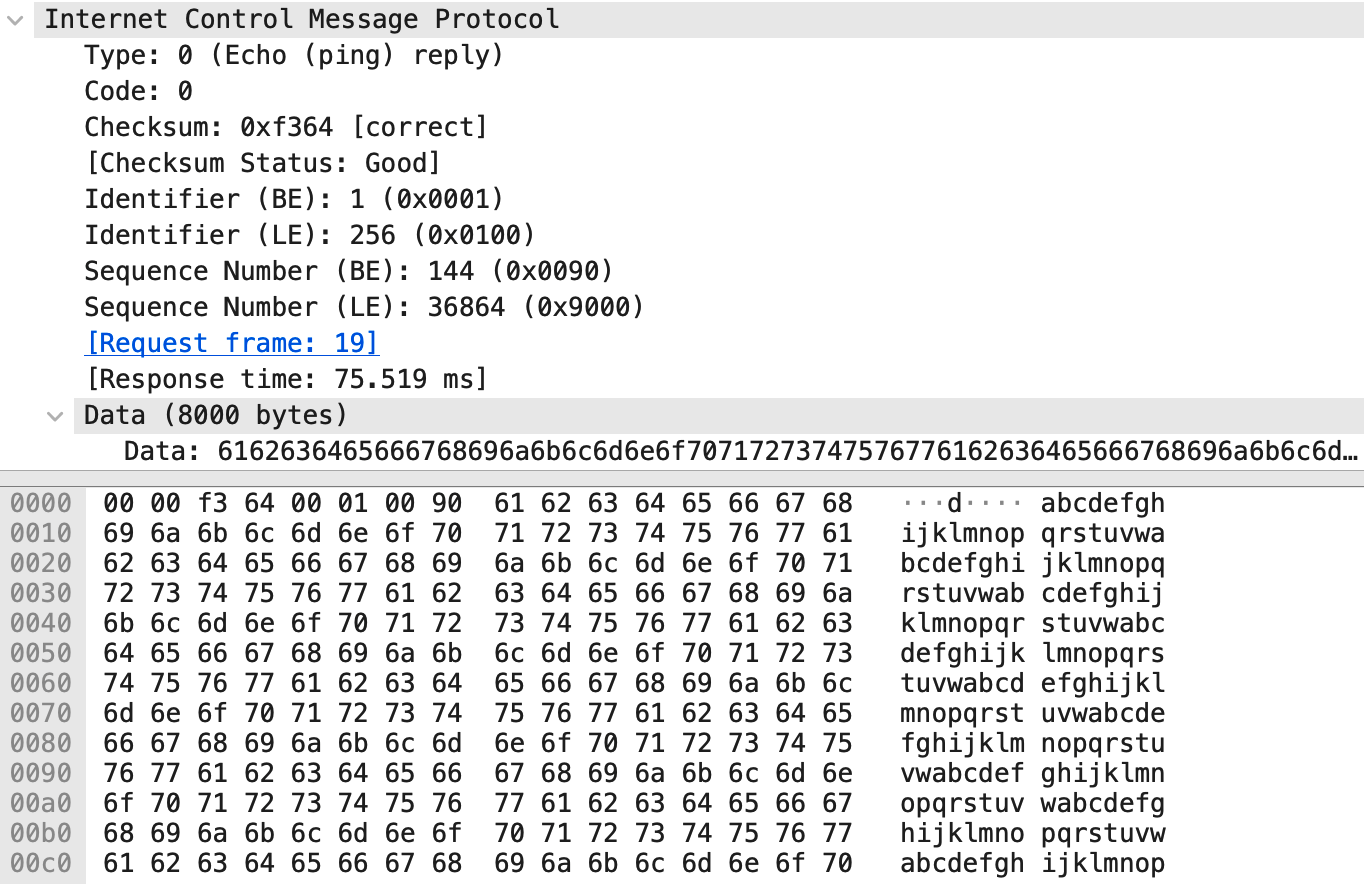
\includegraphics[width=\linewidth]{./Images/ICMP2.png}
        \end{minipage}
    }
    \caption{\mintinline{shell}{ping}命令产生的ICMP分组的内容\label{fig:icmp}}

\end{figure}

序号为19的ICMP分组头的分析如\tabref{tab:icmp1res}。

\begin{table}[!htbp]
    \centering
    \caption{序号为19的ICMP分组头分析\label{tab:icmp1res}}
    \begin{tabular}{|c|c|l|}
        \hline
        字段 (字节数) & 内容(16进制) & 解释 \\
        \hline
        Type (1) & 08 & 类型 \\
        \hline
        Code (1) & 00 & 与Type字段共同构成Control Message:Echo Request \\
        \hline
        Checksum (2) & eb 64 & 校验和:0xeb64 \\
        \hline
        Identifier (2) & 00 01 & 标识符,用于区分不同进程ping消息 \\
        \hline
        Sequence Number (2) & 00 90 & ping请求序号 \\
        \hline
    \end{tabular}
\end{table}

序号为27的ICMP分组是对上一个分组的回复,其分组头除了Type字段改为0,表示Echo Reply,以及校验和发生变化之外,其他和第一个ICMP分组头没有区别。

\subsubsection{捕获tracert命令产生的ICMP分组}

在cmd中输入指令\mintinline{shell}{tracert -d 10.21.245.157},追踪从本机到手机的路由。

运行结果如\figref{fig:tracert}。

\begin{figure}[htbp]
    \centering
    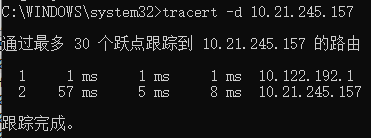
\includegraphics[width=0.5\linewidth]{./Images/tracert.png}
    \caption{\mintinline{shell}{tracert}指令运行结果\label{fig:tracert}}
\end{figure}

在Wireshark过滤器中输入\mintinline{shell}{icmp},过滤出12个分组如\figref{fig:icmps}。其中有三对TTL为1的\mintinline{shell}{ping}请求和回复,还有三对TTL为2的请求和回复。

\begin{figure}[htbp]
    \centering
    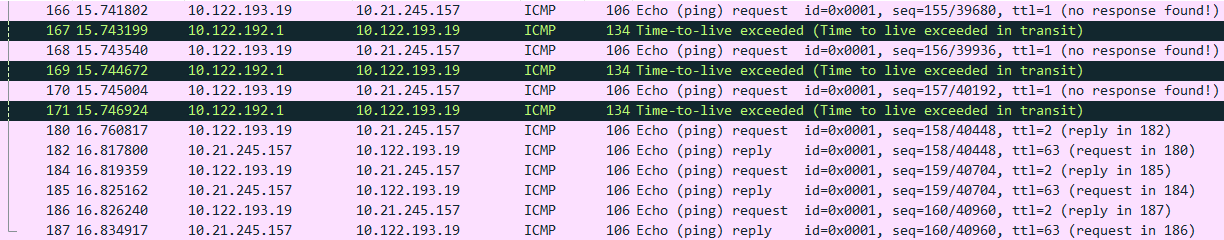
\includegraphics[width=\linewidth]{./Images/ICMP.png}
    \caption{捕获到的12个ICMP分组\label{fig:icmps}}
\end{figure}

其中序号为166、167、10、182的ICMP分组的内容如\figref{fig:ticmp}。

\begin{figure}[htbp]

    \centering
    
    \subfigure[序号为166的ICMP分组]{
        \begin{minipage}[t]{0.45\linewidth}
            \centering
            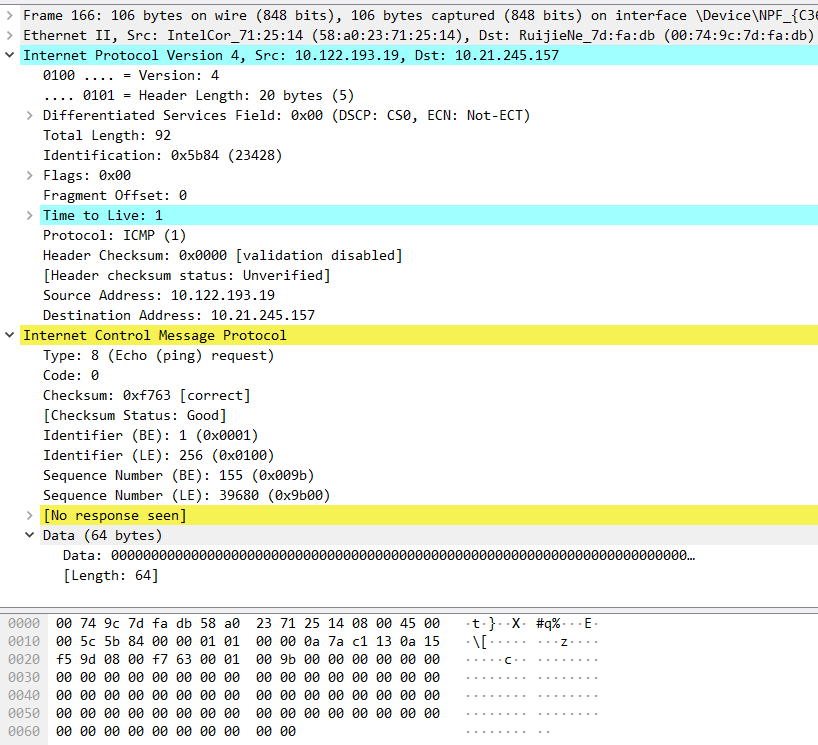
\includegraphics[width=\linewidth]{./Images/ICMP3.png}
        \end{minipage}
    }
    \subfigure[序号为167的ICMP分组]{
        \begin{minipage}[t]{0.45\linewidth}
            \centering
            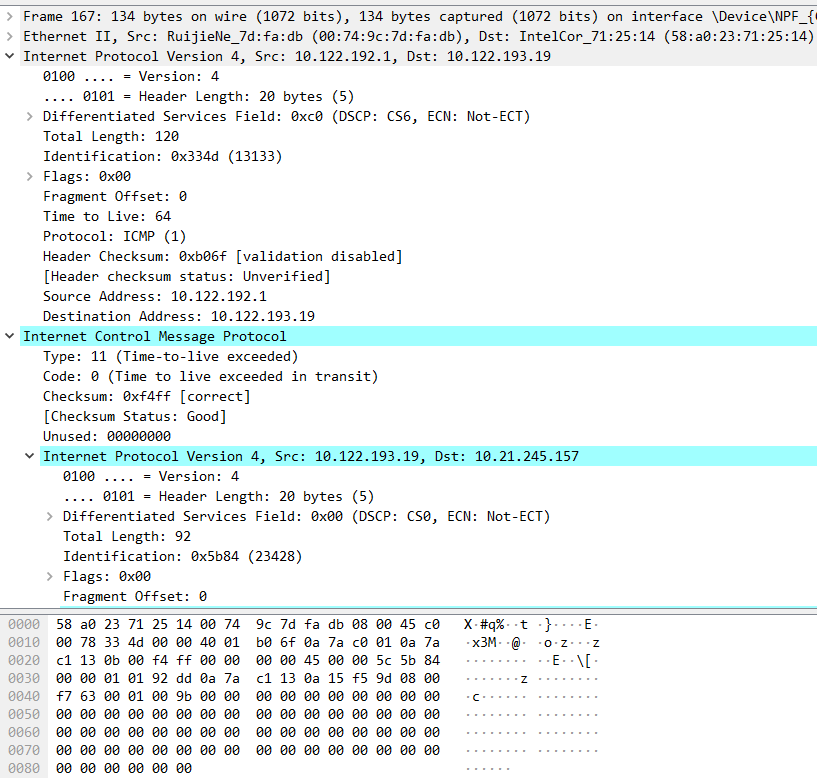
\includegraphics[width=\linewidth]{./Images/ICMP4.png}
        \end{minipage}
    }

    \subfigure[序号为180的ICMP分组]{
        \begin{minipage}[t]{0.45\linewidth}
            \centering
            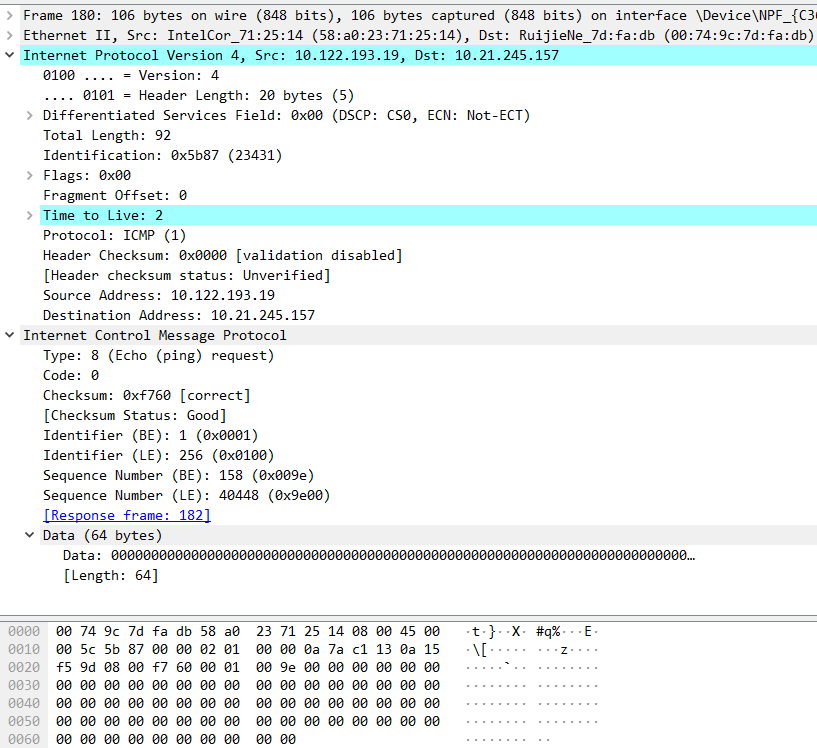
\includegraphics[width=\linewidth]{./Images/ICMP5.png}
        \end{minipage}
    }
    \subfigure[序号为182的ICMP分组]{
        \begin{minipage}[t]{0.45\linewidth}
            \centering
            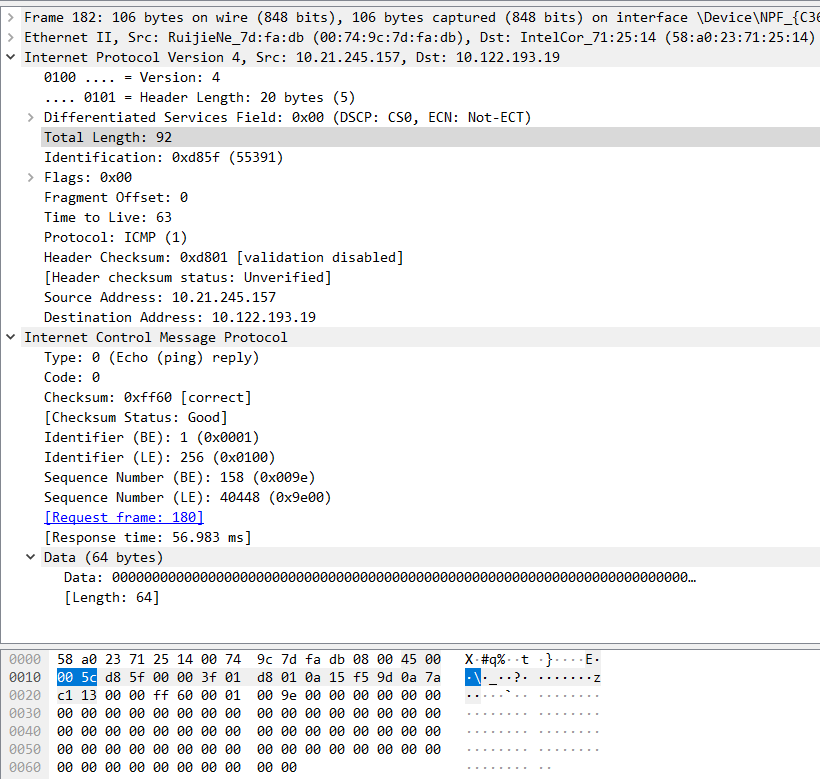
\includegraphics[width=\linewidth]{./Images/ICMP6.png}
        \end{minipage}
    }
    \caption{\mintinline{shell}{tracert}命令产生的ICMP分组的内容\label{fig:ticmp}}

\end{figure}

序号为166的分组的IP部分的TTL为1,ICMP分组头的分析如\tabref{tab:icmp3res}。

\begin{table}[!htbp]
    \centering
    \caption{序号为166的ICMP分组头分析\label{tab:icmp3res}}
    \begin{tabular}{|c|c|l|}
        \hline
        字段 (字节数) & 内容(16进制) & 解释 \\
        \hline
        Type (1) & 08 & 类型 \\
        \hline
        Code (1) & 00 & 与Type字段共同构成Control Message:Echo Request \\
        \hline
        Checksum (2) & f7 63 & 校验和:0xf763 \\
        \hline
        Identifier (2) & 00 01 & 标识符,用于区分不同进程ping消息 \\
        \hline
        Sequence Number (2) & 00 9b & ping请求序号 \\
        \hline
    \end{tabular}
\end{table}

这个分组经过一跳之后,TTL变为0,路由器返回超时信息,即序号为167的分组,其数据部分附带原来分组的的IP头部和8个字节的ICMP头部,其ICMP分组分析如\tabref{tab:icmp4res}。

\begin{table}[!htbp]
    \centering
    \caption{序号为167的ICMP分组分析\label{tab:icmp4res}}
    \begin{tabular}{|c|c|l|}
        \hline
        字段 (字节数) & 内容(16进制) & 解释 \\
        \hline
        Type (1) & 11 & 类型 \\
        \hline
        Code (1) & 00 & 与Type字段共同构成Control Message:TTL expired in transit \\
        \hline
        Checksum (2) & f4 ff & 校验和:0xf4ff \\
        \hline
        - (4) & 00 00 00 00 & 未使用 \\
        \hline
        IPv4报文头 (20) & 略 & 序号为166的分组的IP头 \\ 
        \hline
        ICMP (8) & 略 & 序号为166的分组的ICMP头 \\
        \hline
    \end{tabular}
\end{table}

本机经过两跳之后就能到达手机,于是TTL为2时可以收到回复。序号为180、182的分组的ICMP头分析如\tabref{tab:icmp5res}、\tabref{tab:icmp6res}。

\begin{table}[!htbp]
    \centering
    \caption{序号为180的ICMP分组头分析\label{tab:icmp5res}}
    \begin{tabular}{|c|c|l|}
        \hline
        字段 (字节数) & 内容(16进制) & 解释 \\
        \hline
        Type (1) & 08 & 类型 \\
        \hline
        Code (1) & 00 & 与Type字段共同构成Control Message:Echo Request \\
        \hline
        Checksum (2) & f7 60 & 校验和:0xf760 \\
        \hline
        Identifier (2) & 00 01 & 标识符,用于区分不同进程ping消息 \\
        \hline
        Sequence Number (2) & 00 9e & ping请求序号 \\
        \hline
    \end{tabular}
\end{table}

\begin{table}[!htbp]
    \centering
    \caption{序号为182的ICMP分组头分析\label{tab:icmp6res}}
    \begin{tabular}{|c|c|l|}
        \hline
        字段 (字节数) & 内容(16进制) & 解释 \\
        \hline
        Type (1) & 00 & 类型 \\
        \hline
        Code (1) & 00 & 与Type字段共同构成Control Message:Echo Reply \\
        \hline
        Checksum (2) & ff 60 & 校验和:0xff60 \\
        \hline
        Identifier (2) & 00 01 & 标识符,用于区分不同进程ping消息 \\
        \hline
        Sequence Number (2) & 00 9e & ping请求序号 \\
        \hline
    \end{tabular}
\end{table}

\section{实验总结和心得体会}

完成本实验大约耗费我4个小时的时间,其中主要的时间花费在查阅英文文档上,这使我查找和阅读英文文档的能力有所增强。

调试时,我学习并且灵活运用了Wireshark的筛选功能,从诸多报文中筛选需要的一部分,节省了许多时间。

在本次实验过程中,我主要查阅相关RFC文档、wiki和Wireshark的帮助文档,通过与课本上理论知识联系,对IP、DHCP、ARP、ICMP协议报文的内容和部分功能有了初步的认识,对其作用原理有更深刻的理解。

\end{document}